% 
\documentclass[a4paper]{article}
\usepackage[OT1]{fontenc}
\usepackage{Sweave}
\setkeys{Gin}{width=0.8\textwidth}
\usepackage{hyperref}
\usepackage{booktabs}
\usepackage[left=40mm, right=40mm, top=30mm, bottom=30mm, 
      includefoot, headheight=13.6pt]{geometry} 
      %set margins to be 30mm (needs to include page numbers
\hypersetup{pdfpagelayout=SinglePage} 
% http://www.tug.org/applications/hyperref/ftp/doc/manual.html                                
\hypersetup{
    colorlinks,%
    citecolor=black,%
    filecolor=black,%
    linkcolor=black,%
    urlcolor=black
} % have links but print like standard text 
% http://en.wikibooks.org/wiki/LaTeX/Hyperlinks

\begin{document}
\title{Sweave Example: Item Analysis Report}
\author{Jeromy Anglim}

\maketitle






\begin{abstract}
This document provides an example of using Sweave 
to record console input and output.
Such a format is useful for several purposes including
R tutorials, informal analyses, and analyses that will be consumed
by readers knowledgeable about a specific project and about R.
The example involves performing an item analysis of 
responses of 127 students 
to a set of 50 multiple choice test items.
The test items were developed by students as part of an informal
class exercise.
They are by design of widely varying quality and difficulty.
For a copy and explanation of the source code, go to
\url{http://jeromyanglim.blogspot.com/2010/11/sweave-tutorial-3-console-input-and.html}
\end{abstract}

\section{Import Data}
The following code imports the data,
initial settings, loading needed packages and
loading data and metadata.
\begin{Schunk}
\begin{Sinput}
> options(stringsAsFactors=FALSE)
> options(width=80)
> library(psych) # used scoring and alpha
> library(CTT) # used for spearman brown prophecy
> cases <- read.delim("data/cases.tsv")
> items <- read.delim("meta/items.tsv")
> items$variable <- paste("item", items$item, sep="")
\end{Sinput}
\end{Schunk}


\section{Initial Inspection of Items}
\begin{Schunk}
\begin{Sinput}
> itemstats <- score.multiple.choice(key = items$correct, 
+ 			data = cases[,items$variable])
\end{Sinput}
\end{Schunk}

The following output shows the item,
correct response (key), the proportion
giving response 1, 2, 3, and 4, the item total correlation(r)
the sample size (n), and the proportion correct (mean).
\begin{Schunk}
\begin{Sinput}
> itemstats$item.stats[,c("key", "1", "2", "3", "4", "r", "n", "mean")]
\end{Sinput}
\begin{Soutput}
       key    1    2    3    4     r   n mean
item1    3 0.31 0.09 0.54 0.06  0.13 127 0.54
item2    2 0.03 0.91 0.02 0.04  0.08 127 0.91
item3    4 0.01 0.08 0.01 0.91  0.21 127 0.91
item4    1 0.78 0.02 0.06 0.14  0.23 127 0.78
item5    2 0.31 0.35 0.06 0.27 -0.01 127 0.35
item6    2 0.03 0.90 0.02 0.05  0.25 127 0.90
item7    1 0.69 0.10 0.14 0.07  0.22 127 0.69
item8    1 0.91 0.01 0.01 0.07  0.19 127 0.91
item9    1 0.92 0.05 0.03 0.00  0.43 127 0.92
item10   3 0.02 0.15 0.61 0.21  0.31 127 0.61
item11   4 0.09 0.01 0.02 0.88  0.28 127 0.88
item12   4 0.12 0.28 0.14 0.46  0.12 127 0.46
item13   1 0.98 0.00 0.02 0.00  0.39 127 0.98
item14   2 0.09 0.74 0.13 0.05  0.10 127 0.74
item15   4 0.16 0.06 0.02 0.77  0.40 127 0.77
item16   2 0.06 0.79 0.15 0.01  0.33 127 0.79
item17   4 0.02 0.00 0.02 0.96  0.43 127 0.96
item18   1 0.50 0.35 0.09 0.06  0.28 127 0.50
item19   2 0.02 0.98 0.00 0.00  0.33 127 0.98
item20   4 0.01 0.02 0.01 0.97  0.48 127 0.97
item21   1 0.72 0.02 0.23 0.02  0.35 127 0.72
item22   4 0.01 0.12 0.00 0.87  0.29 127 0.87
item23   2 0.00 1.00 0.00 0.00    NA 127 1.00
item24   1 0.66 0.13 0.01 0.20  0.27 127 0.66
item25   2 0.02 0.52 0.17 0.28  0.15 127 0.52
item26   1 0.97 0.02 0.01 0.00  0.45 127 0.97
item27   2 0.02 0.85 0.11 0.02  0.33 127 0.85
item28   2 0.02 0.91 0.05 0.02  0.28 127 0.91
item29   4 0.00 0.04 0.02 0.94  0.46 127 0.94
item30   2 0.20 0.62 0.08 0.10  0.32 127 0.62
item31   1 0.68 0.10 0.15 0.07  0.22 127 0.68
item32   2 0.07 0.70 0.09 0.13  0.18 127 0.70
item33   4 0.01 0.02 0.01 0.97  0.61 127 0.97
item34   3 0.09 0.20 0.52 0.18  0.29 127 0.52
item35   4 0.02 0.00 0.02 0.96  0.62 127 0.96
item36   1 0.50 0.16 0.09 0.26  0.11 127 0.50
item37   2 0.09 0.68 0.20 0.03  0.14 127 0.68
item38   1 0.44 0.11 0.16 0.29  0.36 127 0.44
item39   2 0.03 0.73 0.17 0.07  0.28 127 0.73
item40   2 0.02 0.93 0.02 0.02  0.36 127 0.93
item41   1 0.95 0.02 0.01 0.02  0.48 127 0.95
item42   4 0.13 0.01 0.06 0.80  0.28 127 0.80
item43   3 0.00 0.06 0.88 0.06  0.44 127 0.88
item44   2 0.23 0.70 0.02 0.06  0.37 127 0.70
item45   1 0.35 0.32 0.12 0.21  0.19 127 0.35
item46   4 0.06 0.20 0.02 0.72  0.08 127 0.72
item47   4 0.06 0.14 0.09 0.70  0.26 127 0.70
item48   1 0.98 0.02 0.00 0.01  0.16 127 0.98
item49   3 0.01 0.38 0.60 0.02  0.19 127 0.60
item50   2 0.05 0.87 0.01 0.07  0.23 127 0.87
\end{Soutput}
\end{Schunk}

Item 23 appears to be easy.
The absence of variability means that item-total correlations 
can not be calculated for this item.
A quick look at the item suggests why this might be the case:

\begin{Schunk}
\begin{Sinput}
> t(items[items$item == 23, ])
\end{Sinput}
\begin{Soutput}
         23      
item     "23"    
text     "1+1"   
option1  "3"     
option2  "2"     
option3  "4"     
option4  "5"     
correct  "2"     
variable "item23"
\end{Soutput}
\end{Schunk}

Using all 50 items the scale has modest reliabilty
(alpha = 0.68).

\begin{Schunk}
\begin{Sinput}
> itemstats$alpha
\end{Sinput}
\begin{Soutput}
[1] 0.68
\end{Soutput}
\end{Schunk}

The following figure plots proportion answering the item
correct by item-total correlation.
The horizontal and vertical lines represent rough rules of thumb
 dividing poorer from better items
 (i.e., those with a mean that differentiates
 and an item-total correlation that suggests that the item
 is measuring a meaningful construct).
Thus, items in the middle upper section might be regarded as better items.

However, several caveats should be mentioned.
(a) these are only sample estimates,
(b) what constitutes a good item depends on purpose,
(c) inferences are best made when the external sample is the
 same as the norm sample.


\begin{Schunk}
\begin{Sinput}
> plot(r ~ mean , itemstats$item.stats, type="n")
> text(itemstats$item.stats$mean, itemstats$item.stats$r, 1:50)
> abline(h=.2, v=c(.5, .9))
\end{Sinput}
\end{Schunk}
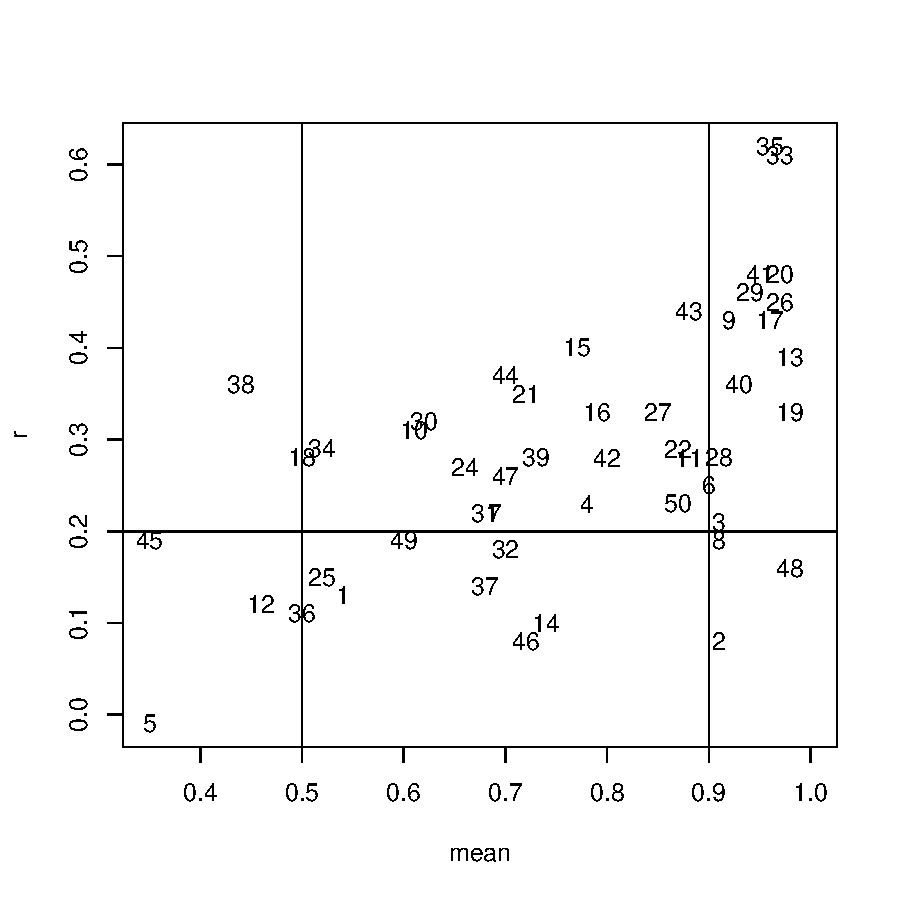
\includegraphics{Item_Analysis_Report-plot_mean_by_r}


Before seeing whether items need deleting,
the distribution of scores are presented.
The stem and leaf plot shows a couple of cases
who performed at close to chance levels.  

\begin{Schunk}
\begin{Sinput}
> scases <- data.frame(score.multiple.choice(key = items$correct, 
+ 			data = cases[,items$variable], score=FALSE))
> scases$correct <-	apply(scases, 1, mean)
> scases$id <- cases$id
> psych::describe(scases$correct)
\end{Sinput}
\begin{Soutput}
  vars   n mean   sd median trimmed  mad  min  max range  skew kurtosis   se
1    1 127 0.77 0.09   0.78    0.77 0.09 0.28 0.92  0.64 -1.94     7.61 0.01
\end{Soutput}
\begin{Sinput}
> stem(scases$correct)
\end{Sinput}
\begin{Soutput}
  The decimal point is 1 digit(s) to the left of the |

  2 | 8
  3 | 2
  3 | 
  4 | 
  4 | 
  5 | 4
  5 | 8
  6 | 444
  6 | 6666668888888
  7 | 0000022222222222222244444444
  7 | 666666666666688888888888888
  8 | 00000002222222222222244444444444
  8 | 666666666888888
  9 | 00002
\end{Soutput}
\end{Schunk}

The id numbers of these cases are shown below.
\begin{Schunk}
\begin{Sinput}
> (outlierIds <- scases[scases$correct < .35, "id"])
\end{Sinput}
\begin{Soutput}
[1]  23 101
\end{Soutput}
\end{Schunk}




\section{Simple Attempt to Improve Scale}
\subsection{Removal of outlier cases}
\begin{Schunk}
\begin{Sinput}
> orcases <- cases[!cases$id %in% outlierIds, ]
> oritemstats <- score.multiple.choice(key = items$correct, 
+ 		data = orcases[,items$variable])
\end{Sinput}
\end{Schunk}

With the outlier cases the scale reliability was estimated to be 
0.68
with the outlier cases removed scale reliability 
was estimated to be 0.48
The lesson to be learnt here is that failure to remove outlier
cases can lead to a gross overestimation of the reliability of a scale.

\subsection{Removal of poor items}
There are many ways of identifying poor items.

\begin{Schunk}
\begin{Sinput}
> rules <- list(
+ 		tooEasy = .95,
+ 		tooHard = .3,
+ 		lowR = .15)
> oritemstats$item.stats$lowR <- 
+ 		oritemstats$item.stats$r < rules$lowR
> oritemstats$item.stats$lowR[is.na(oritemstats$item.stats$lowR)] <- TRUE 
> oritemstats$item.stats$tooEasy <- 
+ 		oritemstats$item.stats$mean > rules$tooEasy
> oritemstats$item.stats$tooHard <- 
+ 		oritemstats$item.stats$mean < rules$tooHard
> oritemstats$item.stats$baditem <-
+ 		with(oritemstats$item.stats,
+ 				(lowR | tooHard | tooEasy))
> baditems <- row.names(oritemstats$item.stats[
+ 						oritemstats$item.stats$baditem, ])
> gooditems <- row.names(oritemstats$item.stats[
+ 						!oritemstats$item.stats$baditem, ])
\end{Sinput}
\end{Schunk}

The code above uses some simple heuristics to flag bad items.
Items were flagged as bad based on the following rules:

\begin{itemize}
\item \emph{Too Easy}: mean correct $>$
0.95.
11
items were bad by this definition.

\item \emph{Too Hard}: mean correct $<$ 
0.3.
0
items were bad by this definition. 

\item \emph{Low Item--Total Correlation}: item total correlation $<$ 
0.15.
15 
items were bad by this definition. 
\end{itemize}

Overall, these three rules flagged 
21 of 
50 items as bad.


The following shows a couple of examples of items flagged as poor
and a couple flagged as good.

\begin{Schunk}
\begin{Sinput}
> oritemstats$item.stats[gooditems[c(1,6)], ]
\end{Sinput}
\begin{Soutput}
       key    1    2    3    4 miss    r   n mean   sd  skew kurtosis   se
item4    1 0.78 0.02 0.05 0.14    0 0.24 125 0.78 0.41 -1.36    -0.14 0.04
item11   4 0.10 0.00 0.02 0.89    0 0.24 125 0.89 0.32 -2.43     3.94 0.03
        lowR tooEasy tooHard baditem
item4  FALSE   FALSE   FALSE   FALSE
item11 FALSE   FALSE   FALSE   FALSE
\end{Soutput}
\begin{Sinput}
> t(items[items$variable == gooditems[1], ])
\end{Sinput}
\begin{Soutput}
         4                                                       
item     "4"                                                     
text     "Select the final number in the sequence 2, 3, 5, 9, __"
option1  "2, 3, 5, 9, 17"                                        
option2  "2, 3, 5, 9, 24"                                        
option3  "2, 3, 5, 9, 27"                                        
option4  "2, 3, 5, 9, 11"                                        
correct  "1"                                                     
variable "item4"                                                 
\end{Soutput}
\begin{Sinput}
> t(items[items$variable == gooditems[6], ])
\end{Sinput}
\begin{Soutput}
         11                                             
item     "11"                                           
text     "What is the best classification for a spider?"
option1  "Insect"                                       
option2  "Animal"                                       
option3  "Crustacean"                                   
option4  "Arachnid"                                     
correct  "4"                                            
variable "item11"                                       
\end{Soutput}
\begin{Sinput}
> oritemstats$item.stats[baditems[c(1,6)], ]
\end{Sinput}
\begin{Soutput}
       key    1    2    3    4 miss    r   n mean  sd  skew kurtosis   se lowR
item1    3 0.31 0.09 0.54 0.06    0 0.06 125 0.54 0.5 -0.17    -1.99 0.04 TRUE
item12   4 0.11 0.28 0.14 0.46    0 0.06 125 0.46 0.5  0.14    -2.00 0.04 TRUE
       tooEasy tooHard baditem
item1    FALSE   FALSE    TRUE
item12   FALSE   FALSE    TRUE
\end{Soutput}
\begin{Sinput}
> t(items[items$variable == baditems[1], ])
\end{Sinput}
\begin{Soutput}
         1                                                                             
item     "1"                                                                           
text     "Choose the most inappropriate answer: \"Hand is to glove, as ___ is to ___ ."
option1  "mouth, food"                                                                 
option2  "finger, ring"                                                                
option3  "foot, shoe"                                                                  
option4  "eye, spectacles"                                                             
correct  "3"                                                                           
variable "item1"                                                                       
\end{Soutput}
\begin{Sinput}
> t(items[items$variable == baditems[6], ])
\end{Sinput}
\begin{Soutput}
         12                                      
item     "12"                                    
text     "In what Australian city is Kings Park?"
option1  "Hobart"                                
option2  "Perth"                                 
option3  "Canberra"                              
option4  "None of the above"                     
correct  "4"                                     
variable "item12"                                
\end{Soutput}
\end{Schunk}

The reliability can then be calculated on the modified scale 
with the items flagged as bad removed.
\begin{Schunk}
\begin{Sinput}
> reditemstats <- score.multiple.choice(
+   key = items[items$variable %in% gooditems, "correct"], 
+ 		data = orcases[,gooditems])
\end{Sinput}
\end{Schunk}

The resulting reliability was 
0.53 up from
0.48.

While this is an improvement, it is still poor.

The Spearman Brown prophecy formula provides a means of
estimating the number of items required to achieve a given alpha. 

\begin{Schunk}
\begin{Sinput}
> sbrown <- list()
> sbrown$targetAlpha <- .8
> sbrown$actualAlpha <- reditemstats$alpha
> sbrown$multiple <- CTT::spearman.brown(sbrown$actualAlpha , .8, "r")$n.new 
> sbrown$refinedItemCount <- nrow(reditemstats$item.stats) * sbrown$multiple
> sbrown$totalItemCount <- nrow(itemstats$item.stats) * sbrown$multiple 
\end{Sinput}
\end{Schunk}

The formula suggests  that in order to obtain
an alpha of 0.8,
3.55 times as many items are required.
Thus, the final scale would need around
103 items.
Assuming a similar number of good and bad items,
this would require an initial pool of around
178 items.  
It should also be noted that these are probably under estimates
given (a) the relatively small sample size, 
and (b) item total correlations
and alpha are likely to be positively biased due to the selection 
procedure used for identifying good test items. 


\section{Conclusion}
If you get a bunch of students 
and give them five minutes to write a bunch of random test items,
don't expect the resulting scale to have
good psychometric properties.  
But of course, this document was intended more as an example of 
using Sweave than as an example of best practice in test construction. 
\end{document}
